\chapter{Εξελικτικοί Αλγόριθμοι} % top level followed by section, subsection

%: ----------------------- paths to graphics ------------------------

% change according to folder and file names
\ifpdf
    \graphicspath{{2/figures/PNG/}{2/figures/PDF/}{2/figures/}}
\else
    \graphicspath{{2/figures/EPS/}{2/figures/}}
\fi

%: ----------------------- contents from here ------------------------

%\begin{flushright}
%Life results from the non-random survival 
%\linebreak
%of randomly varying replicators.
%\linebreak
%Richard Dawkins 
%\end{flushright}
\section{Εισαγωγή}
Στόχος αυτού του κεφαλαίου είναι η παρουσίαση της προϋπάρχουσας υποδομής,  όπως αυτή διαμορφώθηκε στο πλαίσιο προηγούμενων διατριβών στη ΜΠΥΡ\&Β/ΕΘΣ του ΕΜΠ, σχετικής με την ανάπτυξη αποδοτικών μεθόδων βελτιστοποίησης βασισμένων στους ΕΑ \cite{phd_Giotis,phd_Karakasis,phd_Kampolis,phd_Vera,phd_Chara,phd_eugene}.  Η υποδομή αυτή \cite{EASYsite} χρησιμοποιήθηκε ως αλγοριθμική βάση στην παρούσα διδακτορική διατριβή και εμπλουτίστηκε με νέες μεθόδους που παρουσιάζονται αναλυτικά στα επόμενα κεφάλαια, αυξάνοντας ακόμη περισσότερο την ήδη υψηλή απόδοση αυτών. 

Οι EA ανήκουν στην κατηγορία των στοχαστικών, πληθυσμιακών μεθόδων βελτιστοποίησης και μιμούνται τη θεωρία εξέλιξης των ειδών του Δαρβίνου \cite{Darwin}.  Οι πρώτες προσπάθειες χρήσης ΕΑ για την επίλυση προβλημάτων βελτιστοποίησης ξεκίνησαν σχεδόν ταυτόχρονα κατά τα μέσα της δεκαετίας του $1950$, από τους \english{Friedberg} \cite{Friedberg:1958:LMP:1662346.1662347, Friedberg:1959:LMP:1661923.1661930}, \english{Bremermann} \cite{Bremermann_62} και \english{Box} \cite{Box57a}. Στις αρχές της δεκαετίας του $1960$, είχαν διαμορφωθεί οι τρεις κύριες μορφές των ΕΑ οι οποίες, στη συνέχεια, κυριάρχησαν: ο Εξελικτικός Προγραμματισμός (\english{Evolutionary Programming, EP}) από τον \english{Fogel} \cite{fogel62}, οι Στρατηγικές Εξέλιξης (\english{Evolutionary Strategies, ES}) από τον \english{Rechenberg} \cite{rech65} και οι Γενετικοί Αλγόριθμοι (\english{Genetic Algorithms, GA}) από τον \english{Holland} \cite{Holland:1962:OLT:321127.321128}.

Το λογισμικό βελτιστοποίησης \english{EASY (Evolutionary Algorithm System)} της ΜΠΥΡ\&Β/ΕΘΣ κάνει χρήση του προτεινόμενου στην \cite{phd_Giotis} γενικευμένου $(\mu,\lambda)EA$ ο οποίος μπορεί να μετατραπεί, με κατάλληλες ρυθμίσεις, τόσο σε \english{GA} όσο και σε \english{ES}. Οι ακέραιες ποσότητες μ και λ αναφέρονται στο πλήθος των γονέων και απογόνων κάθε γενιάς, αντίστοιχα. Ο $(\mu,\lambda)EA$ χρησιμοποιεί τους τελεστές εξέλιξης (επιλογής γονέων, διασταύρωσης, μετάλλαξης, ελιτισμού) για τη δημιουργία του πληθυσμού των απογόνων.

Τα κύρια πλεονεκτήματα των ΕΑ που τους μετατρέπουν σε ελκυστικά, για τη βιομηχανία, εργαλεία σχεδιασμού-βελτιστοποίησης είναι: α) η ικανότητά τους να εντοπίζουν το καθολικό βέλτιστο, αποφεύγοντας τα τοπικά ακρότατα και β) η ικανότητα τους να χρησιμοποιούν οποιοδήποτε λογισμικό αξιολόγησης χωρίς ανάγκη πρόσβασης στον πηγαίο κώδικα αυτού. Προαπαιτούμενα για την πραγματοποίηση μιας βελτιστοποίησης με χρήση ΕΑ είναι η διαθεσιμότητα λογισμικού αξιολόγησης ικανού να αναλύει κάθε υποψήφια λύση και να ποσοτικοποιήσει την απόδοση/ποιότητά της με βάση τα τεθέντα κριτήρια και την ικανοποίηση των τεθέντων περιορισμών (αν και εφόσον αυτοί υπάρχουν), ο καθορισμός των μεταβλητών σχεδιασμού (και των ορίων τους) και των συναρτήσεων κόστους. 

Η ανάγκη αξιολόγησης όλων των υποψηφίων λύσεων που δημιουργούνται κατά τη διαδικασία της εξέλιξης, ώστε να αποδοθούν σε αυτές οι τιμές των συναρτήσεων κόστους, είναι το αδύνατο σημείο των ΕΑ. Το πρόβλημα γίνεται σημαντικό σε περιπτώσεις όπου το λογισμικό αξιολόγησης έχει υψηλό υπολογιστικό κόστος. Η βελτιστοποίηση μορφής, τόσο στην αεροδυναμική όσο και στην υδροδυναμική, ανήκει σε αυτήν την κατηγορία λόγω της χρήσης κωδίκων ΥΡΔ ως λογισμικού αξιολόγησης. Αυτό αυξάνει αισθητά το χρόνο ολοκλήρωσης της διαδικασίας βελτιστοποίησης. Για να αντιμετωπισθεί η προαναφερθείσα αδυναμία, έχουν αναπτυχθεί τρόποι που α) ελαχιστοποιούν τον αριθμό κλήσεων στο λογισμικό αξιολόγησης, μειώνοντας με αυτόν τον τρόπο το συνολικό υπολογιστικό κόστος της βελτιστοποίησης και β) εκμεταλλεύονται τη διαθεσιμότητα πολυεπεξεργαστικών συστημάτων, αξιολογώντας ταυτοχρόνως πολλές υποψήφιες λύσεις και, έτσι, μειώνοντας το συνολικό χρόνο της αναμονής του σχεδιαστή. Οι δύο αυτές τεχνικές, στις διάφορες παραλλαγές τους, εντάχθηκαν στο λογισμικό \english{EASY} από παλαιότερες διδακτορικές διατριβές της ερευνητικής ομάδας της ΜΠΥΡ\&Β/ΕΘΣ του ΕΜΠ \cite{phd_Giotis,phd_Karakasis,phd_Kampolis,phd_Vera} και μπορούν να χρησιμοποιηθούν σε συνδυασμό με τις προτεινόμενες, σε αυτήν τη διατριβή, μεθόδους. Σχετικές είναι και οι εργασίες \citep{LTT_2_026,LTT_2_045,LTT_2_031,LTT_2_018,LTT_2_020, LTT_2_023, LTT_2_027,LTT_2_029,LTT_2_031, LTT_3_092, LTT_2_053,LTT_2_043} από την ερευνητική ομάδα της ΜΠΥΡ\&Β/ΕΘΣ.               



\section{Βασικές Έννοιες}
Τα προβλήματα βελτιστοποίησης που επιλύονται σε αυτήν τη διατριβή διατυπώνονται γενικά ως προβλήματα ελαχιστοποίησης Μ στόχων και Κ περιορισμών. Μια γενική διατύπωσή τους είναι η  
\label{OPt_def}
\begin{align} 
   &min ~ \vec{F}(\vec{x})=(f_1(\vec{x}),f_2(\vec{x}),...,f_M(\vec{x}))\in \Re^{M} \nonumber \\
   &\mbox{υπό τους περιορισμούς} ~ c_k(\vec{x})\leq d_k, ~~~~~ k =1,K
\label{OptimIN}
\end{align}
όπου $\vec{x}\in X \!\leq\! \Re^{N}$ είναι το διάνυσμα των μεταβλητών σχεδιασμού και $X$ ο χώρος σχεδιασμού. Περιορισμοί ισότητας της μορφής $c^*\left( \vec{x} \right)=d^*$ καλύπτονται από τη διατύπωση \ref{OptimIN} αν γραφούν ως $c\left( \vec{x} \right)= \left|c^*\left( \vec{x} \right) -d^*\right|\!<\!d$, όπου $d\in\mathcal{R}^K$ ένας απειροστά μικρός αριθμός. 



Ο γενικευμένος EA, \cite{phd_Giotis}, που χρησιμοποιήθηκε ως λογισμικό βάσης στην παρούσα διδακτορική διατριβή διαχειρίζεται, σε κάθε γενιά ($g$), τρεις πληθυσμούς: τον πληθυσμό $P_{\lambda}^g$ των $\lambda$ απογόνων, τον $P_{\mu}^g$ των μ γονέων και τον $P_{e}^g$ των $e$ επιλέκτων της γενιάς $g$. Η πιθανότητα επιλογής μίας υποψήφιας λύσης ως γονέα είναι αντιστρόφως ανάλογη της τιμής της προς ελαχιστοποίηση βαθμωτής συνάρτησης κόστους $\Phi$. Η συνάρτηση $\Phi$ ορίζεται στη συνέχεια. Το σύνολο $P_{e}^g$ εμπεριέχει τις καλύτερες, μέχρι στιγμής, λύσεις που ανέδειξε η εξέλιξη.  Ακολουθεί ο αλγόριθμος του γενικευμένου ΕΑ \cite{phd_Giotis}, στη μορφή που καλύπτει τόσο μονοκριτηριακή και πολυκριτηριακή βελτιστοποίηση.  

\begin{itemize}

\item[]{\bf Βήμα 1:} (Αρχικοποίηση) Τίθεται $g\!=\!0$, $P_{e}^{g-1}= \emptyset$ και $P_{\mu}^{g-1}= \emptyset$.
	Κάθε μέλος του συνόλου των απογόνων $P_{\lambda}^g$
	αρχικοποιείται μέσω μίας ομοιόμορφης
	γεννήτριας ψευδοτυχαίων αριθμών\footnote{
	\english{Pseudo Random Number Generator, PRNG.}}	λαμβάνοντας υπόψη τα τεθέντα άνω
	και κάτω όρια των μεταβλητών σχεδιασμού. Ένα, συνήθως μικρό, υποσύνολο του $P_{\lambda}^g$ μπορεί να επιβληθεί εξωτερικά από το χρήστη. Τέτοια άτομα συνήθως αποτελούν βέλτιστες λύσεις παρόμοιων προβλημάτων ή άλλες λύσεις που σέβονται όμως τους περιορισμούς.      

\item[]{\bf Βήμα 2:} (Αξιολόγηση) Κάθε μέλος του συνόλου απογόνων αξιολογείται χρησιμοποιώντας
	το πρότυπο αξιολόγησης, υπολογίζεται δηλαδή το διάνυσμα τιμών
	$\vec{F}(\vec{x}) \in \Re^{M}$, για κάθε $\vec{x} \in P_{\lambda}^g$.
\item[]{\bf Βήμα 3:} (Απόδοση βαθμωτού κόστους) Για κάθε $\vec{x} \in P_{\lambda}^g \cup P_{\mu}^g \cup P_{e}^{g-1}$, υπολογίζεται μια βαθμωτή τιμή κόστους $\Phi(\vec{x})$ συναρτήσει του $\vec{F}(\vec{x})$. Για προβλήματα ενός στόχου $\Phi(\vec{x}) \equiv F(\vec{x})$.
\item[]{\bf Βήμα 4:} (Ανανέωση επιλέκτων) Τα $e^*$ καλύτερα μέλη του $P_{\lambda}^g \cup P_{e}^{g-1}$ επιλέγονται ως μέλη του $P_e^g$. Αν $e^*\!>\!e$, εφαρμόζεται τελεστής αραίωσης \cite{phd_Giotis} για να αφαιρεθούν τα επιπλέον $e^*\!-\!e$ άτομα.     
\item[]{\bf Βήμα 5:} (Ελιτισμός) Μικρός αριθμός επιλέκτων, ο οποίος επιλέγεται τυχαία από το $P_e^g$, αντικαθιστά τα χειρότερα μέλη του $P_{\lambda}^g$.     
\item[]{\bf Βήμα 6:} (Επιλογή γονέων) Τα μέλη του $P_{\mu}^g$ επιλέγονται από το $P_{\lambda}^g \cup P_{\mu}^{g-1}$ λαμβάνοντας υπόψη το επιτρεπόμενο όριο ζωής $\kappa$ (εκφρασμένο σε αριθμό γενιών) κάθε γονέα και απογόνου. Σε συμβολική γραφή, $P_{\mu}^{g}=S(P_{\mu}^{g-1},P_{\lambda}^g,\kappa)$.  
\item[]{\bf Βήμα 7:} (Διασταύρωση \& μετάλλαξη) Η επόμενη γενιά απογόνων $P_{\lambda}^{g+1}$ διαμορφώνεται από το $P_{\mu}^{g}$ κάνοντας χρήση των τελεστών, διασταύρωσης ($\mathcal{R}$) και μετάλλαξης ($\mathcal{M}$). Σε συμβολική γραφή, $P_{\lambda}^{g+1} =\mathcal{M}(\mathcal{R}(P_{\mu}^{g}))$.
\item[]{\bf Βήμα 8:} (Έλεγχος τερματισμού) Αν ικανοποιείται κάποιο από τα τεθέντα κριτήρια σύγκλισης του ΕΑ ο αλγόριθμος τερματίζεται, αλλιώς $g\leftarrow g+1$ και επιστροφή στο βήμα 2.

\end{itemize}

Οι βασικοί ορισμοί συμβόλων που χρησιμοποιούνται στο (μ,λ)ΕΑ παρέχονται στον πίνακα \ref{GEA nomenclature}.

\subsection{Πολυκριτηριακή Βελτιστοποίηση}
\label{MOOini}
Αν $M\!>\!1$, το πρόβλημα (\ref{OptimIN}) είναι ένα πρόβλημα ελαχιστοποίησης πολλών στόχων. Στην περίπτωση που υπάρχει μία λύση $\vec{x}^*$, η οποία συγχρόνως ελαχιστοποιεί όλους τους στόχους, αυτή αποτελεί την καθολικά βέλτιστη λύση του προβλήματος. Στη συνήθη περίπτωση όπου οι στόχοι είναι αντικρουόμενοι, χρησιμοποιείται η έννοια της κυριαρχίας κατά \english{Pareto}, όπως αυτή ορίζεται στη συνέχεια.

Για να γίνει δυνατή η χρήση ενός ΕΑ στην πολυκριτηριακή βελτιστοποίηση είναι απαραίτητη μία εμβόλιμη τεχνική που θα μετατρέπει το διάνυσμα $\vec{F}(\vec{x})$ σε βαθμωτό $\Phi(\vec{x})$. Με τον τρόπο αυτό, όλες οι τεχνικές που αναπτύσσονται για μονοκριτηριακή βελτιστοποίηση εφαρμόζονται και στην πολυκριτηριακή. Στην παρούσα διατριβή, αυτό επιτυγχάνεται κάνοντας χρήση της τεχνικής \english{SPEA2}, \cite{Zitz02,Zitz01}, η οποία βασίζεται στην έννοια της κυριαρχίας κατά \english{Pareto}. Ακολουθούν οι ορισμοί της κυριαρχίας και της βέλτιστης λύσης κατά \english{Pareto}:    

\paragraph{Κυριαρχία κατά \english{Pareto}:} 
     Η λύση $\vec{x}_1\!\in\!X$ κυριαρχεί κατά \english{Pareto} της $\vec{x}_2\!\in\!X$ ($\vec{x}_1\prec\vec{x}_2$) αν και μόνο αν δεν παρουσιάζει χειρότερη (μεγαλύτερη, σε πρόβλημα ελαχιστοποίησης) τιμή για όλες τις συναρτήσεις κόστους, ενώ τουλάχιστον μια από αυτές παρουσιάζει καλύτερη (χαμηλότερη σε πρόβλημα ελαχιστοποίησης) τιμή ως προς την αντίστοιχη της	λύσης $\vec{x}_2$, \cite{Gold89}. Μαθηματικά διατυπωμένο: 
\begin{equation}
    \vec{x}_1\prec\vec{x}_2 \Leftrightarrow (\forall i \in[1,M] :  f_i(\vec{x}_1) \leq f_i(\vec{x}_2))\wedge (\exists _i : f_i(\vec{x}_1) < f_i(\vec{x}_2))
    \label{pareto_eq} 
\end{equation}

\paragraph{Βέλτιστη κατά \english{Pareto} λύση:} 
Μια λύση $\vec{x}_1\!\in\!X$ ($X$ είναι το σύνολο των αποδεκτών λύσεων) είναι βέλτιστη κατά \english{Pareto} αν και μόνο αν δεν κυριαρχείται κατά \english{Pareto} από καμία άλλη λύση $\vec{x}\!\in\!X$, δηλαδή αν και μόνο αν, \cite{Gold89},

\begin{eqnarray}
    \nexists\vec{x}:\vec{x}\prec\vec{x}_1, ~~~~ \vec{x},\vec{x}_1\in X \!\subseteq\! \Re^{N}
\end{eqnarray}


\begin{figure}[h!]
\begin{minipage}[b]{1\linewidth}
 \centering
 \resizebox*{!}{8 cm}{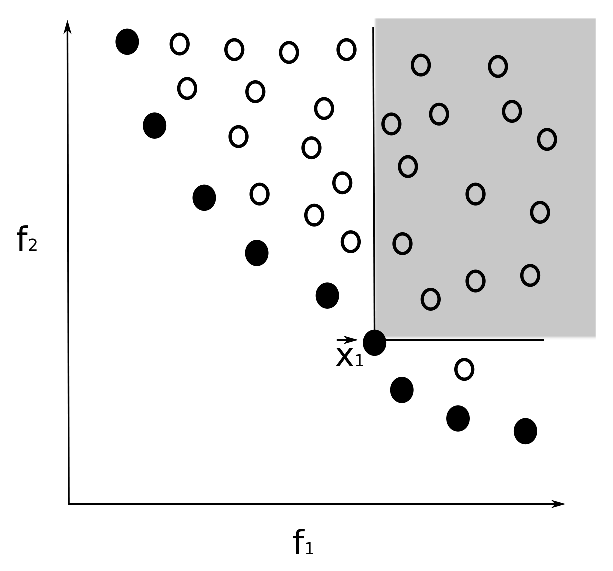
\includegraphics{Pareto2.eps}}
\end{minipage}
\caption{Σχηματική απεικόνιση της κυριαρχίας κατά \english{Pareto} σε πρόβλημα ελαχιστοποίησης δύο στόχων (Μ=2). Η λύση $\vec{x}_1$ είναι βέλτιστη κατά \english{Pareto} καθώς δεν κυριαρχείται από οποιαδήποτε άλλη λύση. Η λύση $\vec{x}_1$, αυτή καθαυτή, κυριαρχεί σε όλες τις λύσεις που υπάρχουν στη σκιασμένη περιοχή. Το μέτωπο των κατά \english{Pareto} βέλτιστων λύσεων, το οποίο εδώ απεικονίζεται με μαύρους κύκλους, δεν είναι υποχρεωτικά συνεχές.} 
\label{Pareto2}
\end{figure}

Ακολουθεί η παρουσίαση της τεχνικής $SPEA2$, \cite{Zitz02,Zitz01}, που χρησιμοποιείται για να μετατρέψει τα διανύσματα τιμών $F$ των μελών του τρέχοντος πληθυσμού σε βαθμωτές τιμές $\Phi$, με βάση την έννοια της κυριαρχίας κατά \english{Pareto}. Η $SPEA2$ αποδίδει σε κάθε άτομο μια βαθμωτή τιμή αντιπροσωπευτική της αλληλοκυριαρχίας των ατόμων της ένωσης των συνόλων $P_{\lambda}^g$, $P_{\mu}^g$ και $P_{e}^{g-1}$.   

\begin{itemize}
\item[]{\bf Βήμα 1:}  (Υπολογισμός δύναμης) Για κάθε μέλος ($i$) του πληθυσμού 
\newline
	$P=P_{\lambda}^g \cup P_{\mu}^g \cup P_{e}^{g-1}$
	υπολογίζεται η τιμή της δύναμης
		$S_i = \frac{\sum(j : j \in P \wedge i \prec j)} {\sum P}$. Σύμφωνα με τη σχέση αυτή, η δύναμη ενός μέλους $i$ ορίζεται ως το πλήθος των μελών του πληθυσμού στα οποία κυριαρχεί, διαιρεμένο με το συνολικό μέγεθος του πληθυσμού $P$.     

\item[]{\bf Βήμα 2:}  (Υπολογισμός πυκνότητας) Για κάθε μέλος $i$
	του πληθυσμού υπολογίζεται η τιμή πυκνότητας $D_i = \frac{1} {a_i+2}$, ως συνάρτηση της απόστασής του $a_i= min (\parallel \vec{F_i} - \vec{F_k} \parallel)$ από το κοντινότερο μέλος του πληθυσμού. 
	
\item[]{\bf Βήμα 3:}  (Υπολογισμός $\Phi$) 
Η βαθμωτή τιμή κόστους υπολογίζεται για κάθε άτομο του πληθυσμού και ορίζεται ως το άθροισμα
	$\Phi_i = R_i+D_i$
όπου 
\newline
$R_i=\sum _{j \in P \wedge i \prec j}|S_j|$ είναι μια βοηθητική ποσότητα (\english{raw fitness}) 
ίση με το άθροισμα της δύναμης των ατόμων από τα οποία κυριαρχείται το υπόψη άτομο. Μεγάλες τιμές της ποσότητας $R_i$ υποδηλώνουν ότι το άτομο κυριαρχείται από πολλά άλλα άτομα. Τα μέλη του μετώπου \english{Pareto} λαμβάνουν εξ ορισμού μηδενική τιμή ($R_i=0$).
\end{itemize}


\subsection{Βελτιστοποίηση με Περιορισμούς}
\label{COPini}
Στην πλειονότητα τους, τα προβλήματα βελτιστοποίησης, κυρίως αυτά που αφορούν σε βιομηχανικές εφαρμογές, πρέπει να ικανοποιούν και ένα σύνολο περιορισμών. Οι περιορισμοί μπορεί να σχετίζονται με γεωμετρικά χαρακτηριστικά ή λειτουργικές επιδόσεις λ.χ. της σχεδιαζόμενης στροβιλομηχανής.  Σε αυτήν τη διατριβή, οι 
ΕΑ 
\newline
αντιμετωπίζουν τα προβλήματα με περιορισμούς κάνοντας χρήση συναρτήσεων ποινής (\english{penalty functions} \cite{Deb00,morales98}).   

Οι όροι ποινής είναι ανάλογοι του κατά πόσο παραβιάζεται ο κάθε περιορισμός και προστίθενται στην $\Phi$. Για κάθε περιορισμό, εκτός της τιμής του κατωφλίου $d_k$ της σχέσης \ref{OptimIN}, ορίζεται επιπλέον και μια «χαλαρωμένη» τιμή $d_k^*\!>\!d_k$. Στην περίπτωση που το άτομο υπερβεί το «χαλαρωμένο» κατώφλι $d_k^*$, τότε αυτομάτως αποδίδεται «ποινή θανάτου» (\english{death penalty}), η οποία πρακτικά ισοδυναμεί με «άπειρη» τιμή της ποσότητας $\Phi$. Στην περίπτωση που κανένας περιορισμός δεν υπερβαίνει το «χαλαρωμένο» όριο, η τιμή της $\Phi$ υπολογίζεται από τη σχέση:
     
\begin{eqnarray}
	\Phi(\vec{x})=\Phi(\vec{x})+ \prod _{k=1}^K{\left\{ 				\begin{array}{ll}
    exp(a_k\frac{c_k(x)-d_k}{d_k^* -d_k}) & ~~,c_k(x)>d_k\\
    1 & ~~,c_k(x)\leq d_k\end{array} \right. }
    \label{penal2}
\end{eqnarray}
όπου οι συντελεστές $a_k$ καθορίζονται από το χρήστη και ρυθμίζουν τη σημαντικότητα κάθε περιορισμού.


\begin{table}[htdp]
\centering
\begin{tabular}{lr} 
\hline
\hline
Πλήθος μεταβλητών σχεδιασμού & N\\
Πλήθος στόχων & M\\
Πλήθος περιορισμών   & K\\
\hline
Υποψήφια λύση, διάνυσμα μεταβλητών σχεδιασμού   & $\vec{x}=(x_1,...,x_N)$\\
Συνάρτηση-στόχος &$f_i(\vec{x})$ \\
Διάνυσμα στόχων (αν Μ$>\!1$)  &$\vec{F}=(f_1(\vec{x}),...,f_M(\vec{x}))$\\
Συνάρτηση-περιορισμός &$c_i(\vec{x})$ \\
Διάνυσμα περιορισμών  & $\vec{C}=(c_1(\vec{x}),...,c_K(\vec{x}))$\\
Βαθμωτή συνάρτηση κόστους & $\Phi$ \\
\hline
Πλήθος απογόνων ανά γενιά &   $\lambda$ 			\\
Πλήθος γονέων ανά γενιά&  $\mu$ 				\\
Πλήθος επιλέκτων ανά γενιά&  $e$			\\
Διάρκεια ζωής ατόμου (μετρούμενη σε γενιές)&  $\kappa$			\\
Πλήθος γονέων που σχηματίζουν έναν απόγονο &  $\rho$			\\
\hline
\hline
\end{tabular}
\caption{Γενικευμένος Εξελικτικός Αλγόριθμος $(\mu,\lambda)$EA: Βασικοί Συμβολισμοί.}
\label{GEA nomenclature} 
\end{table}



\section{ΕΑ Υποβοηθούμενοι από Μεταπρότυπα}
Η αντικατάσταση του ακριβούς προτύπου αξιολόγησης (λ.χ. του κώδικα ΥΡΔ στις εφαρμογές αερο- ή υδροδυναμικής) με κάποιο άλλο πρότυπο αξιολόγησης  (μεταπρότυπο/\english{metamodel}), το οποίο έχει αρκετά μικρότερο υπολογιστικό κόστος και, συνήθως, είναι μια γενική μέθοδος παρεμβολής ή προσέγγισης, είναι η βασική ιδέα των υποβοηθούμενων από μεταπρότυπα ΕΑ (\english{Metamodel-Assisted Evolutionary Algorithms} ή ΜΑΕΑ).

Σε αυτήν τη διατριβή χρησιμοποιούνται ΕΑ με μεταπρότυπα συνδεόμενα με την εξέλιξη μέσω της τεχνικής της προσεγγιστικής προ-αξιολόγησης (ΠΠΑ), \english{Inexact Pre--Evaluation (IPE)}, \cite{phd_Giotis,phd_Karakasis,phd_Kampolis,phd_Vera,LTT_2_018,LTT_2_044}. Η φάση της ΠΠΑ ξεκινά όταν στη βάση δεδομένων του ΕΑ έχει αρχειοθετηθεί ένας ελάχιστος αριθμός (ορίζεται από το χρήστη) αξιολογημένων υποψήφιων λύσεων.  Κατά τη φάση της ΠΠΑ, εκπαιδεύ-ονται $(\lambda\!-\!\lambda^*)$ μεταπρότυπα, όπου $\lambda^*$ ο αριθμός των ατόμων του τρέχοντος πληθυσμού που υπάρχουν ήδη στη βάση δεδομένων. Ασφαλώς,  αυτά τα $\lambda^*$ άτομα δεν χρειάζεται να αξιολογηθούν, για την απόδοση προσεγγιστικής τιμής κόστους $\Phi^*$ στις $(\lambda\!-\!\lambda^*)$ υποψήφιες λύσεις. Κάθε μεταπρότυπο δίνει μια εκτίμηση της τιμής της συνάρτησης-στόχου του αντίστοιχου ατόμου. Με αυτήν την έννοια, τα μεταπρότυπα χαρακτηρίζονται ως «τοπικά» (\english{local metamodels}). Τέλος, τα $\lambda_e$ καλύτερα άτομα του πληθυσμού, με βάση τις αποδοθείσες τιμές  $\Phi^*$, προκρίνονται για αξιολόγηση με το ακριβές πρότυπο, εδώ το λογισμικό ΥΡΔ. Λεπτομερέστερη περιγραφή της τεχνικής ΠΠΑ βρίσκεται στο Κεφάλαιο $2$ του πλήρους κειμένου. Το σχήμα \ref{MAEA} σκιαγραφεί ένα ΜΑΕΑ. 

\begin{figure}[h!]
\centering
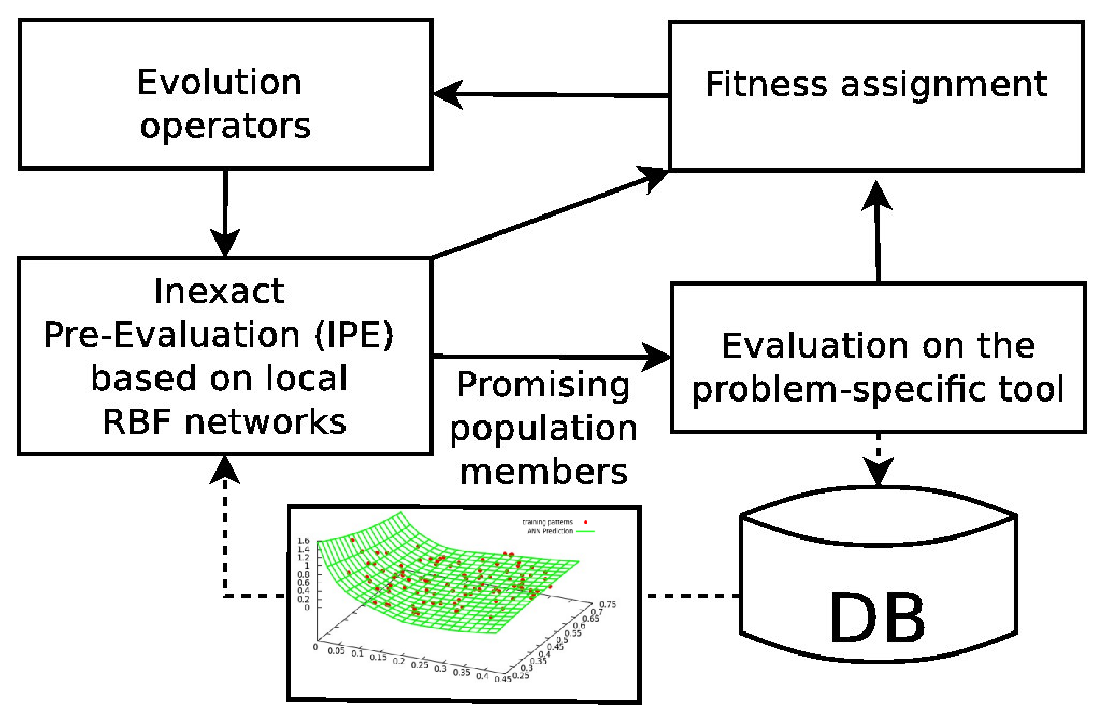
\includegraphics[width=100mm]{MAEA.eps} 
\caption{Ο ΜΑΕΑ με μεταπρότυπα συνδεδεμένα με την εξέλιξη μέσω της τεχνικής της προσεγγιστικής προ-αξιολόγησης (ΠΠΑ).}
\label{MAEA}
\end{figure}

Στην παρούσα διατριβή, ως μεταπρότυπα χρησιμοποιούνται τεχνητά νευρωνικά δίκτυα (ΤΝΔ, \english{Artificial Neural Networks, ANN)} και, συγκεκριμένα, Δίκτυα Συναρτήσεων Ακτινικής Βάσης \english{(Radial Basis Function networks, RBF)} \cite{Haykin}.

Ένα τυπικό δίκτυο \english{RBF}, με Ν εισόδους και μία έξοδο, κατάλληλο για την πρόβλεψη τιμής μιας συνάρτησης κόστους φαίνεται στο σχήμα \ref{rbf1}. Η συνάρτηση ενεργοποίησης που χρησιμοποιήθηκε είναι η $
	G(u,r)=exp(\frac{-u^2}{r^2})$  
όπου  $u=\Vert \vec{x}-\vec{c}_l \Vert_2$ είναι η απόσταση από το $l^{o}$ κέντρο $\vec{c}_l$ της συνάρτησης ακτινικής βάσης.

\begin{figure}[h!]
\centering
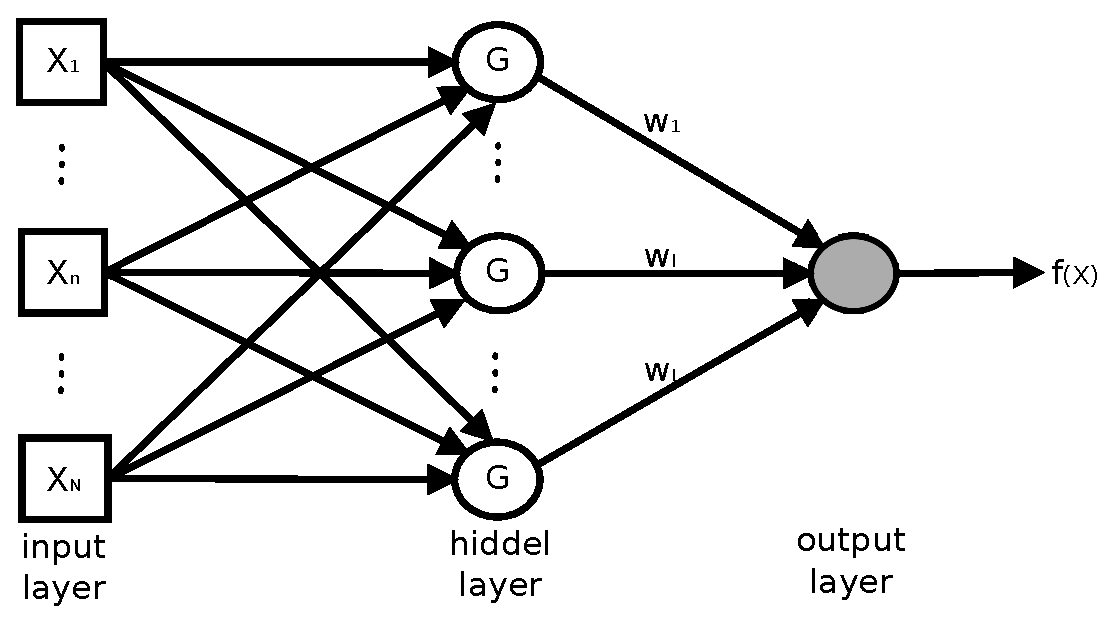
\includegraphics[width=100mm]{RBF.eps} 
\caption{Δίκτυο συναρτήσεων ακτινικής βάσης Ν εισόδων και μίας εξόδου, το οποίο χρησιμοποιείται ως μεταπρότυπο του ΜΑΕΑ της παρούσας διατριβής.}
\label{rbf1}
\end{figure}

%Η έξοδος του ΔΑΒ υπολογίζεται απο:
%\begin{eqnarray}
%	f(x)=\sum _1^K w_i*G(u(x_i),r)
%\label{response}
%\end{eqnarray}         
%\label{MAEApar}
%\newpage
\section{Ιεραρχική-Πολυεπίπεδη Βελτιστοποίηση} 

Η επίλυση ενός προβλήματος βελτιστοποίησης σε έναν αριθμό «επιπέδων βελτιστοποίησης», χρησιμοποιώντας στο κάθε επίπεδο: α) υπολογιστικά εργαλεία αξιολόγησης των υποψήφιων λύσεων διαφορετικού κόστους και ακρίβειας, β) μεθόδους ανίχνευσης διαφορετικού τύπου, ενδεχομένως στοχαστικές σε κάποια επίπεδα και αιτιοκρατικές σε άλλα, γ) παραμετροποίηση της προς σχεδιασμό μορφής με διαφορετικούς βαθμούς ελευθερίας,  αποτελεί τη βασική ιδέα της ιεραρχικής (\english{Hierarchical EA, HEA}) ή πολυεπίπεδης βελτιστοποίησης, \cite{phd_Kampolis,LTT_2_031,LTT_2_044,LTT_3_094,LTT_3_095}. 


Οι προαναφερθείσες μορφές ιεραρχικής-πολυεπίπεδης βελτιστοποίησης (σχήμα \ref{allheas}) μπορούν να χρησιμοποιηθούν ανεξάρτητα ή σε συνδυασμό, χρησιμοποιώντας δύο ή περισσότερα επίπεδα. 


\begin{figure}[h!]
    \centering
    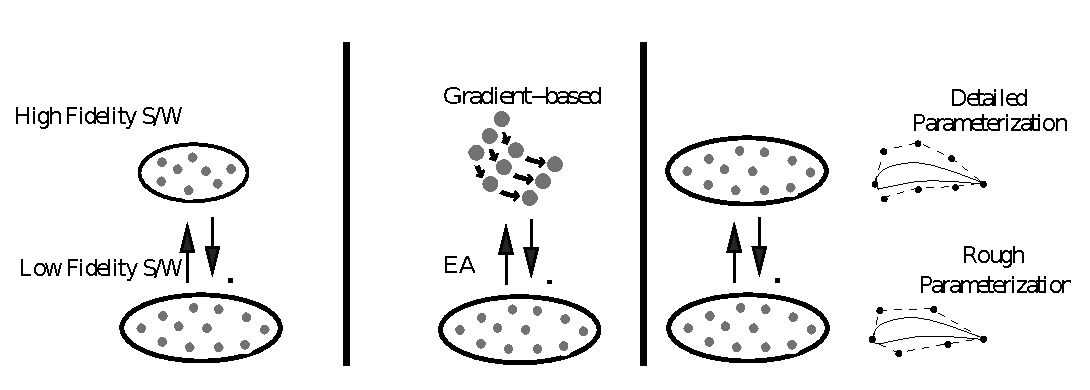
\includegraphics[scale=0.8]{multimodes.eps}
    \caption{Σχηματική απεικόνιση των τριών τύπων ιεραρχικής-πολυεπίπεδης βελτιστοποίησης. Παρουσιάζεται η πλέον συνηθισμένη διεπίπεδη μορφή του προαναφερθέντος γενικού τρόπου σε τρεις εναλλακτικές διατυπώσεις, \cite{phd_Kampolis}.}
    \label{allheas}
\end{figure}      

Στο σχήμα \ref{allheas}, αριστερά, απεικονίζεται ο πολυεπίπεδος (διεπίπεδος ΕΑ) με ιεραρχική αξιολόγηση (\english{Hierarchical Evaluation}). Χρησιμοποιεί λογισμικό χαμηλού υπολογιστικού κόστους και πιστότητας στο χαμηλό επίπεδο και λογισμικό υψηλού κόστους και πιστότητας στο υψηλό επίπεδο, το οποίο χειρίζεται μικρότερο πληθυσμό. Στο μέσο, απεικονίζεται παραλλαγή βασισμένη στην ιεραρχική ανίχνευση (\english{Hierarchical Search}) που υλοποιείται συνήθως εφαρμόζοντας ΕΑ στο χαμηλό επίπεδο και αιτιοκρατικές μεθόδους βελτιστοποίησης στο υψηλό επίπεδο. Τέλος, δεξιά, απεικονίζεται μια τρίτη παραλλαγή που βασίζεται στην ιεραρχική παραμετροποίηση (\english{Hierarchical Parameterization}). Αυτή συνδυάζει την αδρή παραμετροποίηση της προς σχεδιασμό μορφής με λίγες μεταβλητές σχεδιασμού στο χαμηλό επίπεδο με τη λεπτομερή παραμετροποίησή της, με όλους τους βαθμούς ελευθερίας, στο υψηλό επίπεδο.

Η ιεραρχική βελτιστοποίηση δεν χρησιμοποιείται στις εφαρμογές που παρουσιάζει η διατριβή αυτή. Η χρήση των εδώ προτεινόμενων τεχνικών μείωσης του υπολογιστικού κόστους είναι, όμως, άμεσα επεκτάσιμη και στην περίπτωση που χρησιμοποιείται ιεραρχικός ΕΑ. Το κέρδος από τις νέες μεθόδους αναμένεται να υπερτίθεται σε αυτό των ιεραρχικών ΕΑ.



%--------------------------------------------------------------------------
% ----------------------- end of thesis sub-document ------------------------
% ---------------------------------------------------------------------------